\section{Sur-apprentissage}

\subsection{Identification du sur-apprentissage sur les courbes de co\^ut}
Dans le cadre de l'apprentissage supervis\'e, le sur-apprentissage d\'esigne une situation dans laquelle l'optimisation de la loss empirique sur l'ensemble d'apprentissage se poursuit alors que la qualit\'e de g\'en\'eralisation se d\'egrade sur l'ensemble de validation. Si l'on note $L_{\mathrm{app}}^{(t)}$ et $L_{\mathrm{val}}^{(t)}$ les co\^uts observ\'es \`a l'epoch $t$ sur les ensembles d'apprentissage et de validation, le signe caract\'eristique du sur-apprentissage est la poursuite de la d\'ecroissance de $L_{\mathrm{app}}^{(t)}$ alors que $L_{\mathrm{val}}^{(t)}$ recommence \`a cro\^itre apr\`es un minimum. Cette divergence traduit une am\'elioration de l'ajustement aux donn\'ees vues sans gain de g\'en\'eralisation sur les donn\'ees non utilis\'ees pour la mise \`a jour des poids \cite{manzanera_classification_apprentissage,poly_chap4_classifml}.

Pour quantifier ce ph\'enom\`ene, la pr\'esente section retient l'indicateur
\begin{equation}
\Delta_{\mathrm{sur}}
=
L_{\mathrm{val}}^{(T)}
-
\min_{1 \leq t \leq T} L_{\mathrm{val}}^{(t)},
\label{eq:section7_overfit_increase}
\end{equation}
o\`u $T$ d\'esigne l'epoch final du protocole. Une valeur positive de $\Delta_{\mathrm{sur}}$ indique que la loss de validation finale est sup\'erieure \`a son meilleur niveau atteint pendant l'apprentissage. Plus cette quantit\'e est grande, plus la d\'egradation de g\'en\'eralisation en fin d'entra\^inement est marqu\'ee. Le ph\'enom\`ene est d'autant plus probable que la capacit\'e du mod\`ele est \'elev\'ee, que le corpus d'apprentissage est r\'eduit et que la dur\'ee d'entra\^inement est prolong\'ee sans r\'egularisation explicite \cite{poly_chap4_classifml}.

\subsection{Exemple issu du workflow de la Section~6}
La Section~6 fournit d\'ej\`a un exemple exploitable sans introduire de nouvelle architecture. Le \textit{screening} du mod\`ele $M2$ (\textit{three-stage CNN} non r\'egularis\'e), ex\'ecut\'e avec la graine $42$ pendant $10$ epochs, pr\'esente un comportement de sur-apprentissage net. La figure~\ref{fig:section7_overfitting_example} montre que la loss d'apprentissage d\'ecro\^it presque monotoniquement, de $2.0646$ \`a $0.5822$, tandis que la loss de validation atteint un minimum de $1.6178$ \`a l'epoch $4$ avant de remonter jusqu'\`a $2.5590$ \`a l'epoch $10$. Il en r\'esulte
\begin{equation}
\Delta_{\mathrm{sur}} = 2.5590 - 1.6178 = 0.9412.
\end{equation}

Le m\^eme diagnostic appara\^it sur les accuracies : l'accuracy d'apprentissage finale atteint $78.96\%$, alors que l'accuracy finale de validation reste \`a $43.60\%$, soit un \'ecart de $35.36$ points. La meilleure accuracy de validation, $48.20\%$, est d'ailleurs obtenue avant la fin de l'entra\^inement. Ce run constitue donc un exemple pertinent pour illustrer la distinction entre optimisation r\'eussie de l'objectif d'apprentissage et d\'egradation de la g\'en\'eralisation.

\begin{figure}[htbp]
\centering
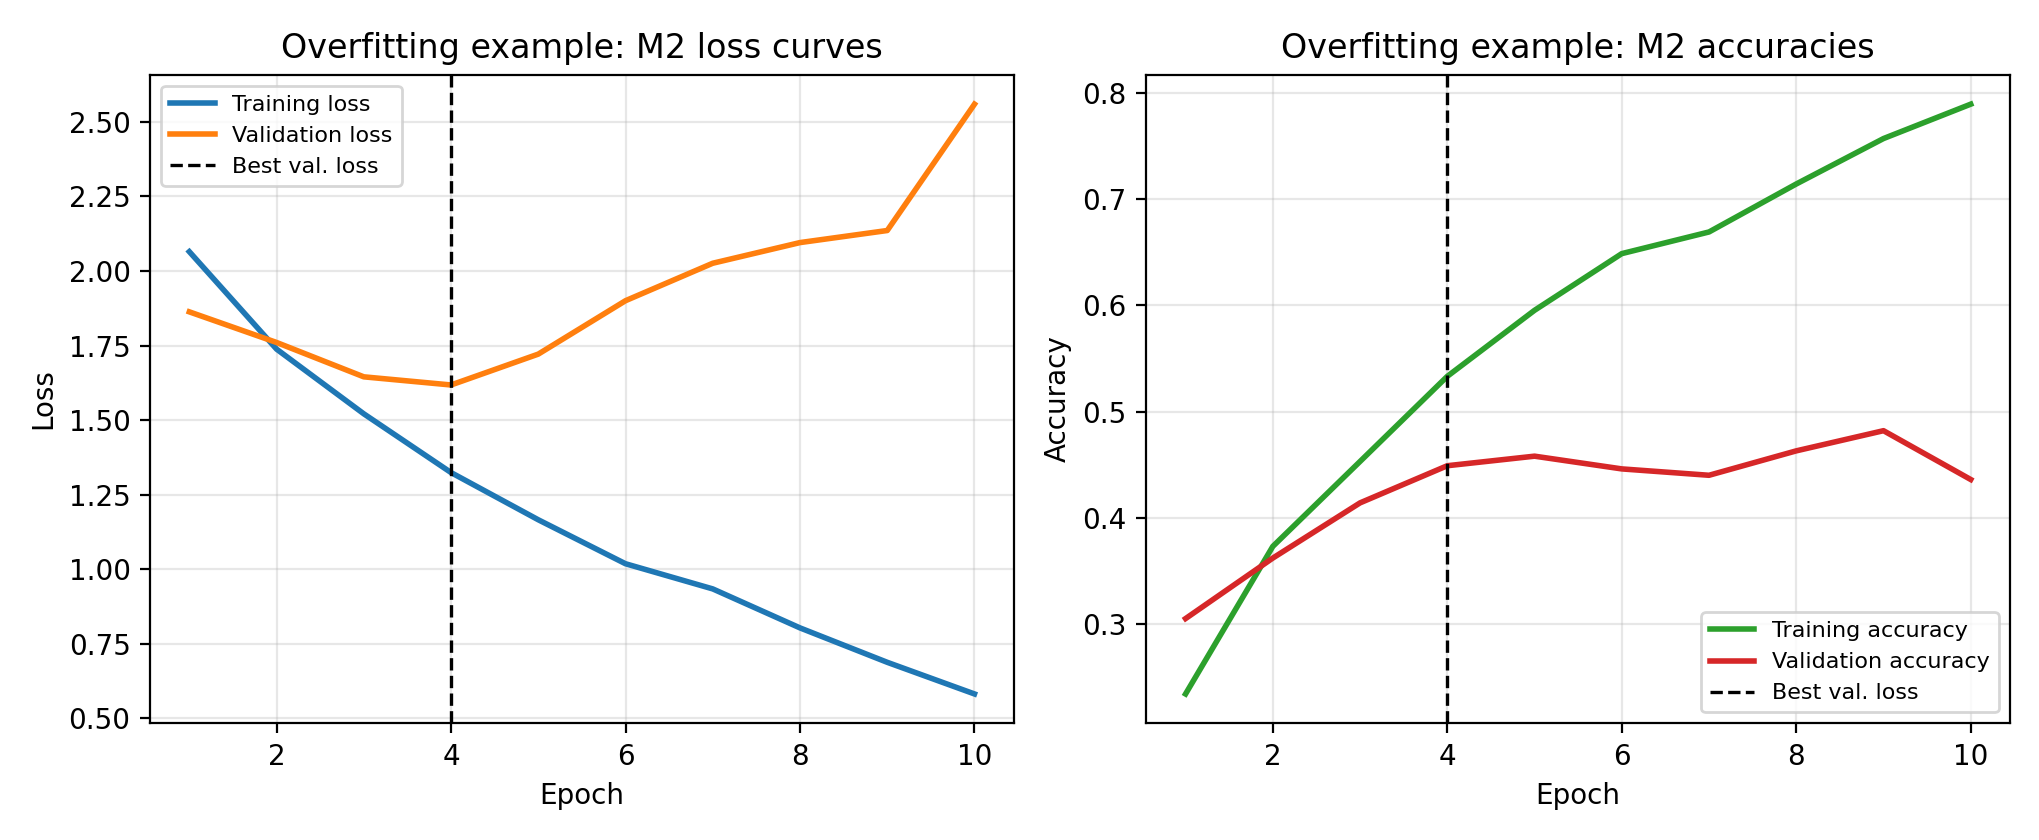
\includegraphics[width=\linewidth]{imgs/section7_overfitting_example.png}
\caption{Exemple de sur-apprentissage r\'eutilis\'e depuis la Section~6 : mod\`ele $M2$, graine $42$, $10$ epochs. Le texte interne \`a la figure est laiss\'e en anglais pour garantir un rendu stable.}
\label{fig:section7_overfitting_example}
\end{figure}

\subsection{Effet de m\'ecanismes de r\'egularisation}
Afin d'\'etudier des m\'ecanismes susceptibles de r\'eduire ce ph\'enom\`ene, une campagne contr\^ol\'ee a \'et\'e men\'ee sur le m\^eme backbone profond que celui de $M2$. Le protocole reste identique \`a celui de la Section~6 : m\^eme split CIFAR-10 r\'eduit ($5000/1000/1000$), m\^eme standardisation image par image, Adam avec $(\epsilon,\beta_1,\beta_2,\eta)=(10^{-3},0.9,0.999,10^{-7})$, \textit{batch size} $32$, \texttt{shuffle=True}, graines $42$ et $314$, et budget fix\'e \`a $15$ epochs. Quatre variantes ont \'et\'e compar\'ees :
\begin{itemize}
\item $R0$ : backbone $M2$ sans r\'egularisation explicite ;
\item $R1$ : backbone $M2$ avec \textit{dropout} ($0.25$ apr\`es chaque \textit{pooling}, $0.5$ avant la couche dense) ;
\item $R2$ : backbone $M2$ avec seule p\'enalisation $L^2$ de coefficient $10^{-4}$ ;
\item $R3$ : mod\`ele $M3$ de la Section~6, combinant \textit{dropout} et p\'enalisation $L^2$.
\end{itemize}

Ces choix correspondent \`a deux m\'ecanismes de r\'egularisation explicitement discut\'es dans le cours. Le \textit{dropout} limite la co-adaptation des neurones en supprimant al\'eatoirement une partie des activations pendant l'apprentissage, alors que la p\'enalisation $L^2$ contraint la norme des poids et d\'ecourage des solutions trop fortement ajust\'ees au corpus d'apprentissage \cite{manzanera_classification_apprentissage,poly_chap4_classifml}. La figure~\ref{fig:section7_regularization_comparison} et le tableau~\ref{tab:section7_regularization} r\'esument les effets observ\'es.

\begin{table*}[htbp]
\centering
\caption{Comparaison des m\'ecanismes de r\'egularisation sur le backbone profond de la Section~6. Le symbole $\pm$ d\'esigne l'\'ecart-type empirique sur les deux graines.}
\label{tab:section7_regularization}
\small
\begin{tabular}{|c|l|c|c|c|c|}
\hline
Variante & M\'ecanisme & Accuracy finale val. (\%) & Min. val. loss & $\Delta_{\mathrm{sur}}$ & \'Ecart final train-val (pts) \\
\hline
$R0$ & aucune & $47.30 \pm 2.00$ & $1.6192 \pm 0.0014$ & $1.3744 \pm 0.0740$ & $43.87 \pm 1.37$ \\
$R1$ & dropout & $53.90 \pm 1.80$ & $1.2743 \pm 0.0636$ & $0.0211 \pm 0.0152$ & $5.58 \pm 0.34$ \\
$R2$ & $L^2$ seul & $48.55 \pm 2.05$ & $1.6630 \pm 0.0763$ & $1.8604 \pm 0.0397$ & $41.79 \pm 0.13$ \\
$R3$ & dropout + $L^2$ & $55.50 \pm 1.10$ & $1.3410 \pm 0.0246$ & $0.0000 \pm 0.0000$ & $3.70 \pm 0.38$ \\
\hline
\end{tabular}
\end{table*}

\begin{figure}[htbp]
\centering
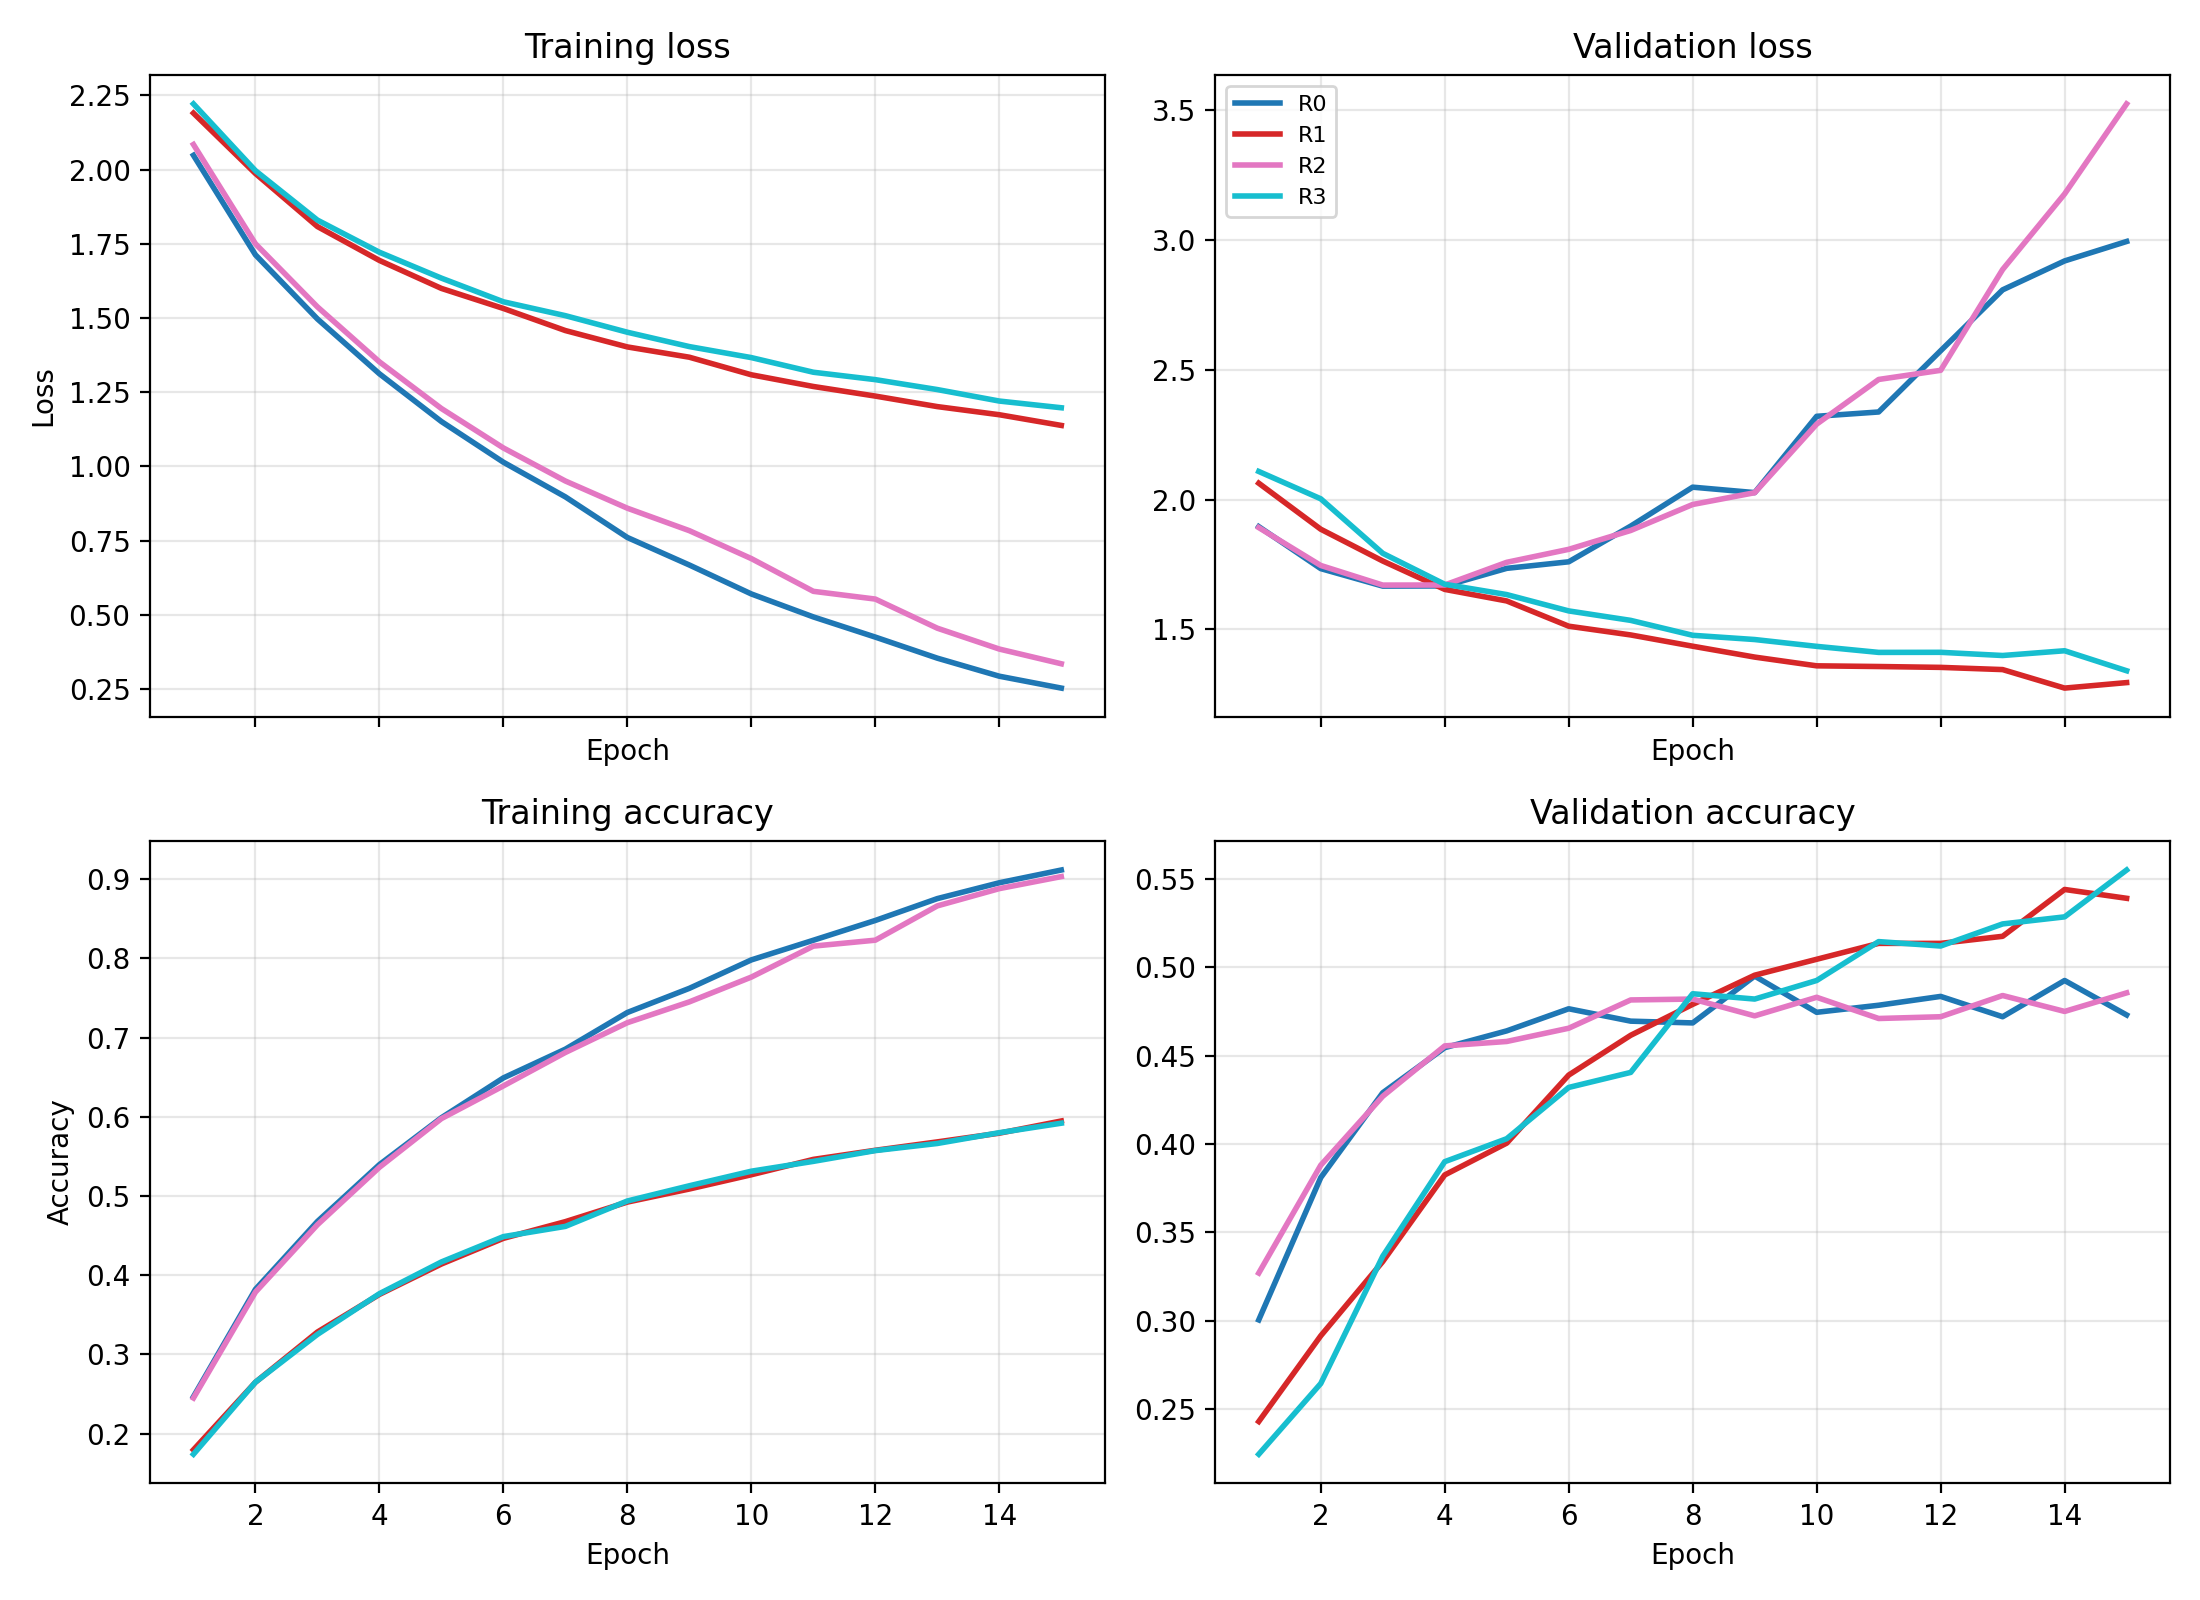
\includegraphics[width=\linewidth]{imgs/section7_regularization_comparison.png}
\caption{Comparaison des courbes moyennes d'apprentissage et de validation pour les variantes $R0$ \`a $R3$. Le texte interne \`a la figure est laiss\'e en anglais pour garantir un rendu stable.}
\label{fig:section7_regularization_comparison}
\end{figure}

\begin{figure}[htbp]
\centering
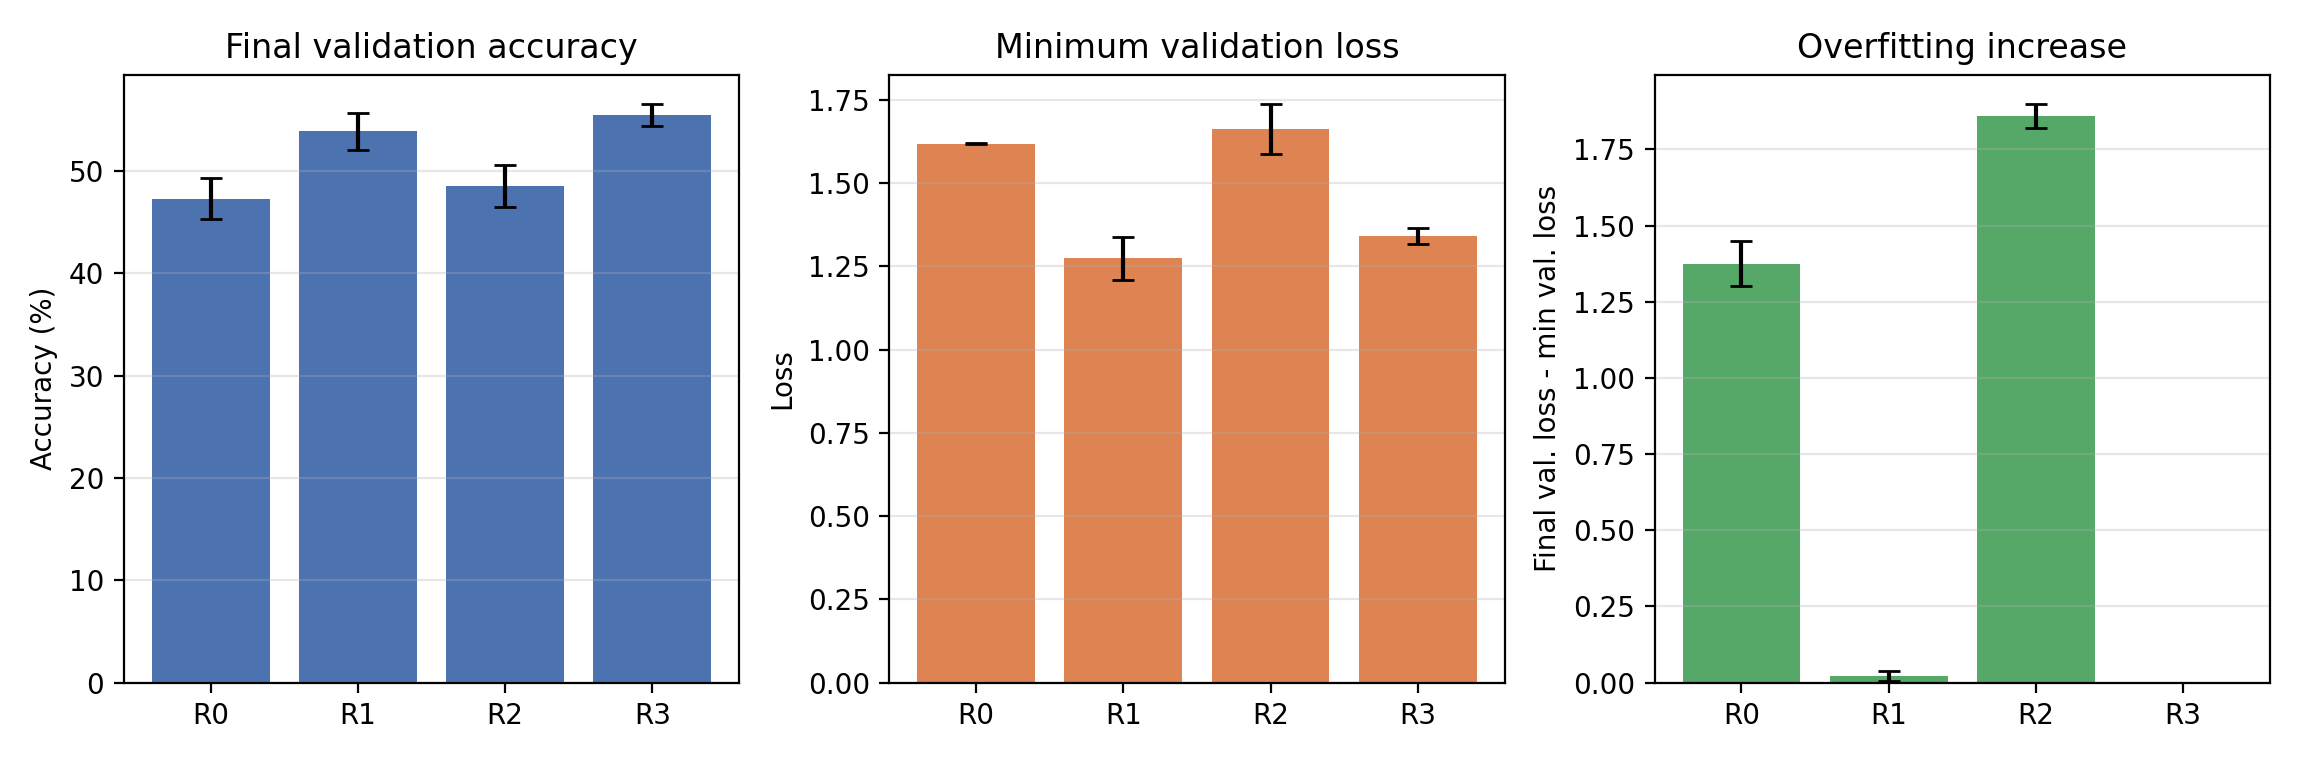
\includegraphics[width=\linewidth]{imgs/section7_regularization_summary.png}
\caption{Synth\`ese graphique des effets observ\'es sur l'accuracy finale de validation, le minimum de \textit{val. loss} et l'indicateur $\Delta_{\mathrm{sur}}$.}
\label{fig:section7_regularization_summary}
\end{figure}

Le comportement de $R0$ confirme le diagnostic initial : la loss d'apprentissage continue de d\'ecro\^itre jusqu'\`a $0.2536$, alors que la loss de validation remonte jusqu'\`a $2.9937$ apr\`es un minimum moyen de $1.6192$. L'indicateur moyen $\Delta_{\mathrm{sur}}=1.3744$ et l'\'ecart final train-val de $43.87$ points t\'emoignent d'une g\'en\'eralisation fortement d\'egrad\'ee. L'ajout du seul \textit{dropout} dans $R1$ modifie radicalement cette dynamique : la loss de validation reste presque monotone jusqu'\`a l'epoch $14$, et $\Delta_{\mathrm{sur}}$ chute \`a $0.0211$. Cette r\'egularisation ralentit l'optimisation sur l'ensemble d'apprentissage, puisque l'accuracy finale train n'est plus que de $59.48\%$, mais elle am\'eliore nettement la validation, avec $53.90\%$ d'accuracy finale et le meilleur minimum moyen de \textit{val. loss} ($1.2743$).

La p\'enalisation $L^2$ seule, test\'ee dans $R2$, ne produit pas le m\^eme effet sous ce protocole. L'accuracy finale de validation, $48.55\%$, reste proche de $R0$, tandis que $\Delta_{\mathrm{sur}}$ atteint $1.8604$, soit une d\'egradation encore plus forte que pour la baseline non r\'egularis\'ee. Cette observation indique que, dans ce cadre exp\'erimental, le coefficient $10^{-4}$ ne suffit pas \`a contenir le sur-apprentissage du backbone profond lorsqu'il est utilis\'e sans \textit{dropout}. Enfin, la combinaison des deux m\'ecanismes dans $R3$ donne le meilleur compromis global : l'accuracy finale de validation atteint $55.50\%$, l'\'ecart train-val tombe \`a $3.70$ points et la loss de validation continue \`a d\'ecro\^itre jusqu'\`a l'epoch final, ce qui conduit \`a $\Delta_{\mathrm{sur}}=0$ sur le budget fix\'e \`a $15$ epochs.

\subsection{Discussion comparative}
Les r\'esultats montrent que la lecture des courbes de co\^ut fournit un crit\`ere de diagnostic plus fiable que la seule observation de l'accuracy finale. Dans les variantes non suffisamment r\'egularis\'ees, l'optimisation du co\^ut d'apprentissage se poursuit alors que la loss de validation se d\'egrade, ce qui signale un apprentissage trop sp\'ecifique aux donn\'ees vues. Ce comportement appara\^it tr\`es clairement pour $M2$ dans l'exemple issu de la Section~6, puis pour $R0$ et $R2$ dans la comparaison contr\^ol\'ee.

La comparaison met aussi en \'evidence que tous les m\'ecanismes de r\'egularisation ne se valent pas dans le protocole retenu. Le \textit{dropout} r\'eduit fortement la co-adaptation et am\'eliore d\'ej\`a nettement la g\'en\'eralisation lorsqu'il est utilis\'e seul. La p\'enalisation $L^2$ de coefficient $10^{-4}$, en revanche, ne suffit pas \`a elle seule \`a stabiliser la validation pour ce backbone et ce budget d'entra\^inement. La combinaison des deux m\'ecanismes fournit finalement le meilleur compromis entre limitation du sur-apprentissage et performance finale, en prolongeant la d\'ecroissance de la loss de validation jusqu'\`a la fin du protocole.

Ces observations restent coh\'erentes avec la Section~6. L'augmentation de profondeur am\'eliore la capacit\'e de repr\'esentation du mod\`ele, mais elle accro\^it aussi le risque de sur-ajustement sur un sous-ensemble d'apprentissage limit\'e \`a $5000$ images. Dans ce contexte, l'introduction de \textit{dropout} et d'une p\'enalisation $L^2$ ne constitue pas un raffinement optionnel, mais une condition importante pour exploiter utilement la capacit\'e suppl\'ementaire du backbone profond. Une strat\'egie telle que l'\textit{early stopping} pourrait encore \^etre mobilis\'ee pour arr\^eter l'entra\^inement au voisinage du minimum de validation, mais elle n'a pas \'et\'e retenue ici afin de conserver un budget d'epochs identique pour toutes les variantes compar\'ees.
